\chapter{Summary statistics}
\label{ch:summary-statistics}

After a purely qualitive inspection of the data, we can now move on to
a more quantitative description. This chapter will introduce a number
of \emph{summary statistics} to summarise larger datasets using just a
few numerical values, including:

\begin{enumerate}
  \item a measure of \emph{location}, representing the `average' of
    the data;
  \item a measure of statistical \emph{dispersion}, quantifying the
    spread of the data; and
  \item a measure of the \emph{shape} of the distribution.
\end{enumerate}

Before proceeding with this topic, it is useful to bear in mind that
these summary statistics have limitations.  The Anscombe quartet of
Table~\ref{tab:anscombe} and Figure~\ref{fig:anscombe} showed that
very different looking datasets can have identical summary
statistics. But with this caveat in mind, summary statistics are an
essential component of data analysis provided that they are preceded
by a visual inspection of the data.

\section{Location}
\label{sec:location}

There are many ways to define the `average' value of a multi-value
dataset.  In this chapter, we will introduce three of these but later
chapters will introduce a few more.

\begin{enumerate}
\item{\bf Mean.} Given a dataset $x = \{x_1,\ldots ,x_i,\ldots, x_n\}$
  comprising $n$ values, the arithmetic mean ($\bar{x}$) is defined
  as:
  \begin{equation}
    \bar{x} = \frac{1}{n}\sum\limits_{i=1}^{n}x_i
    \label{eq:mean}
  \end{equation}
\item{\bf Median.} The median is obtained by ranking the observations
  according to size, and selecting the middle value. If $n$ is an odd
  number, then:
  \begin{equation}
    \mbox{med}(x) = x_1 < \ldots < {\bf x_{(n+1)/2}} < \ldots < x_n
  \end{equation}

  If $n$ is an even number, then the median is the average of the two
  numbers on either side of the middle. Graphically, the median can be
  identified as the value that corresponds the to halfway point of the
  ECDF.
  
\item{\bf Mode.} For discrete datasets, the mode is the most
  frequently occurring value. For continuous datasets, it can be
  roughly identified as the steepest region on the ECDF, or as the
  highest point on a histogram or KDE. Note that the outcome of the
  latter procedure may depend on the histogram bandwidth or KDE
  bandwidth.
\end{enumerate}

Applying these three concepts to the pH data, the mean is given by:
\begin{equation*}
  \bar{x} = \frac{
    \begin{array}{c}
      6.2+4.4+5.6+5.2+4.5+5.4+4.8+5.9+3.9+4.0+ \\
      5.1+4.1+5.1+5.5+5.2+4.6+5.7+4.6+4.6+5.6
    \end{array}
  }{20} = 5.00
\end{equation*}

The median is obtained by ranking the values in increasing order, and
marking the two middle values in bold:

\begin{center}
  {3.9, 4.0, 4.1, 4.4, 4.5, 4.6, 4.6, 4.6, 4.8, \textbf{5.1},
  \textbf{5.1}, 5.2, 5.2, 5.4, 5.5, 5.6, 5.6, 5.7, 5.9, 6.2}
\end{center}

Then the median is the average of these two values (median[x] =
5.1). The most frequently occurring pH value in the dataset is 4.6,
but this is a rounded value from a continuous distribution. If instead
we use a KDE to identify the mode, then this yields a value of 5.3:

\noindent\begin{minipage}[t][][b]{.5\textwidth}
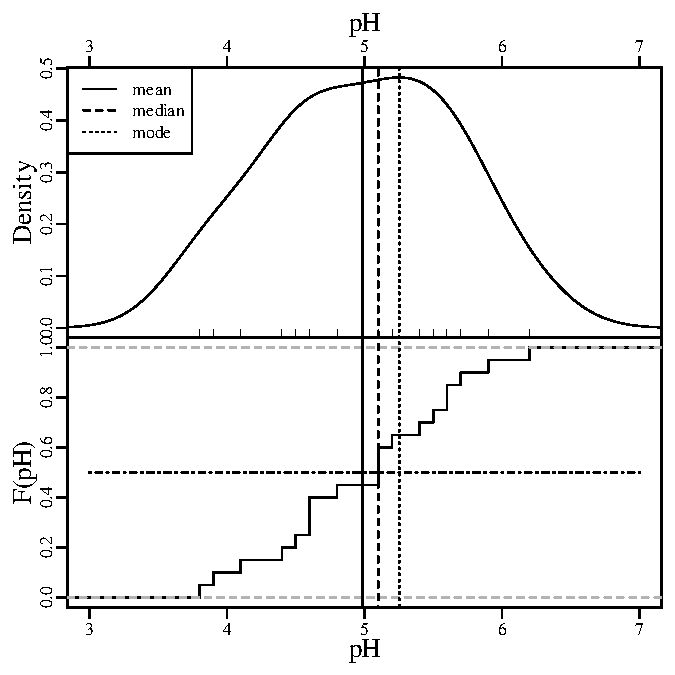
\includegraphics[width=\textwidth]{../figures/pHlocation.pdf}
\end{minipage}
\begin{minipage}[t][][t]{.5\textwidth}
  \captionof{figure}{KDE (top) and ECDF (bottom) of the pH data (mean
    = 5.0, median = 5.1, mode = 5.3). The dash-dot line on the bottom
    panel marks halfway mark of the ECDF. The intersection of this
    line with the ECDF marks the median. For this dataset, all three
    measures of location are closely spaced together in the densest
    sampling area.}
\end{minipage}

Calculating the same three summary statistics for the Ca/Mg data:

\noindent\begin{minipage}[t][][b]{.5\textwidth}
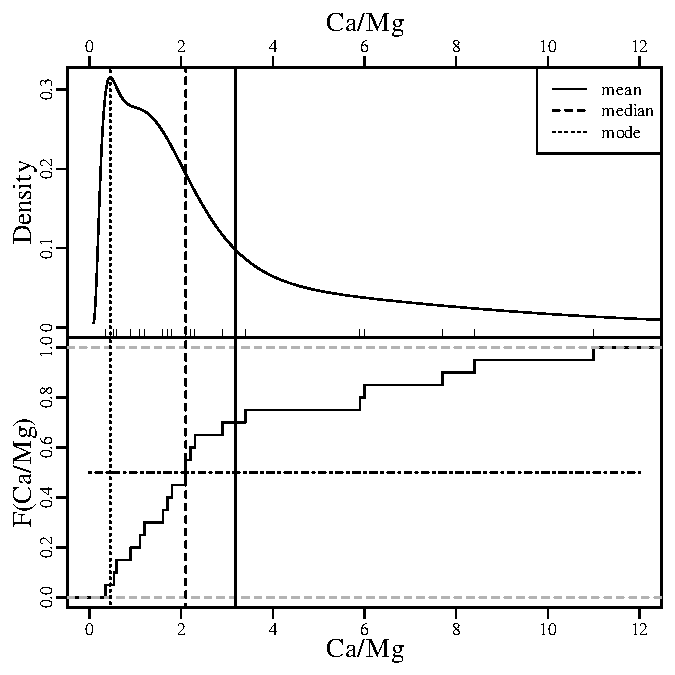
\includegraphics[width=\textwidth]{../figures/CaMglocation.pdf}
\end{minipage}
\begin{minipage}[t][][t]{.5\textwidth}
  \captionof{figure}{KDE and ECDF of the Ca/Mg data (mean = 3.2, median
    = 2.1, mode = 0.45). The mean is strongly affected by the long
    `tail' of large outliers. It is 7 times greater than the
    mode. Only 6 out of 20 catchments (30\%) are larger than the mean
    of the distribution and only 1 (5\%) is smaller than the mode.}
  \label{fig:CaMglocation}
\end{minipage}
\vfill Finally, repeating the exercise one more time for the
vegetation and geyser eruption data:

\noindent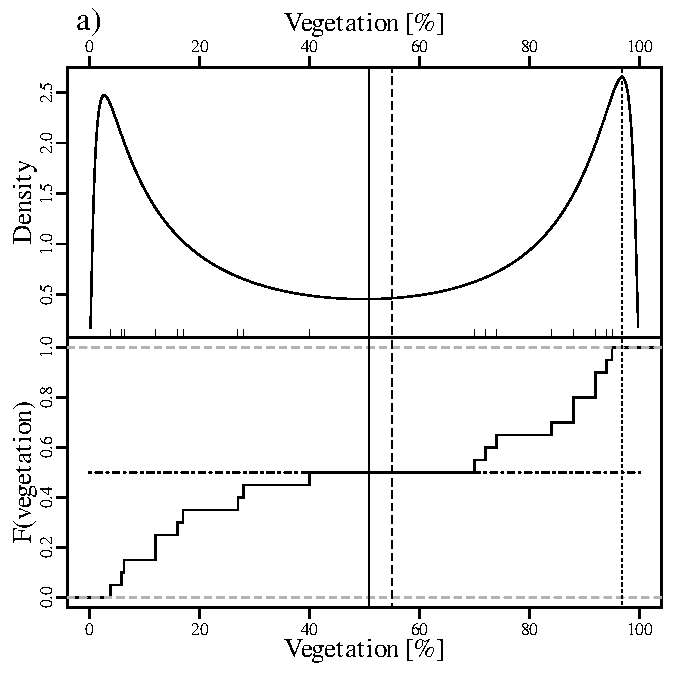
\includegraphics[width=.5\textwidth]{../figures/vegetationlocation.pdf}
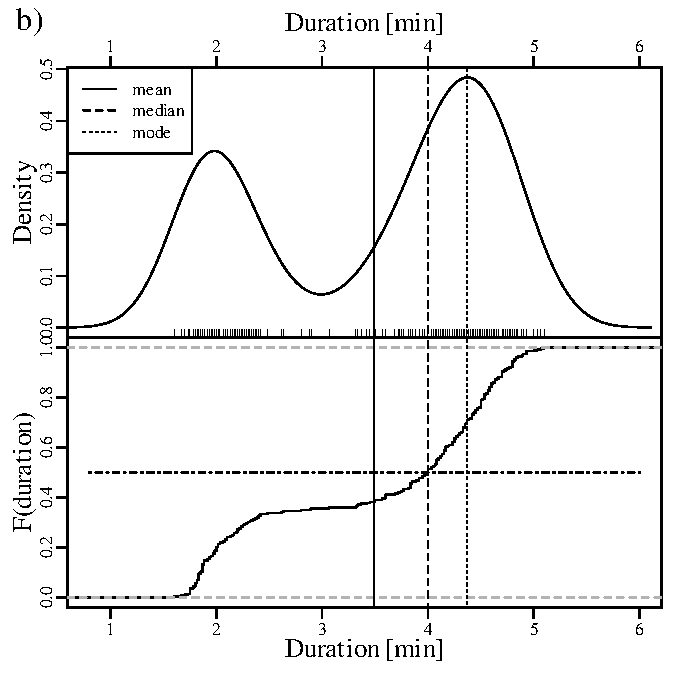
\includegraphics[width=.5\textwidth]{../figures/eruptionslocation.pdf}
\begingroup \captionof{figure}{KDE and ECDF of a) the vegetation data
  (mean = 0.51, median = 0.55, mode = 0.97); and b) the geyser
  eruption data (mean = 3.5, median = 4.0, mode = 4.4). Both of
  these distributions are `bimodal', meaning that they have two
  `peaks' in the KDE, corresponding to two steep segments in the
  ECDFs. The dotted lines mark the highest one of them and ignores the
  other one. The mean and median fall in between the two modes and are
  not representative of the data.\medskip}
\label{fig:vegetationlocation}
\endgroup

Comparing the three sets of examples leads to the following
conclusions:

\begin{enumerate}
\item the mean is a meaningful measure of location for unimodal and
  symmetric distribution;
\item the mean is strongly affected by outliers whereas the median is
  not;
\item therefore the median is a more robust estimator of location for
  asymmetric datasets than the mean;
\item multimodal datasets cannot be adequately summarised with a
  single location parameter.
\end{enumerate}

\section{Dispersion}
\label{sec:dispersion}

It is rare for all the values in a dataset to be exactly the same. In
most cases they are spread out over a range of values. The amount of
spread can be defined in a number of ways, the most common of which
are:

\begin{enumerate}

\item{\bf Standard deviation.} Given $n$ measurements $x_i$ (for $1
  \leq i \leq n$), the standard deviation is defined as:
\begin{equation}
  s[x] = \sqrt{\frac{1}{n-1}\sum\limits_{i=1}^{n}(x_i-\bar{x})^2}
  \label{eq:stdev}
\end{equation}

\noindent where $\bar{x}$ is the arithmetic mean
(Equation~\ref{eq:mean}). The square of the standard deviation
(i.e. $s[x]^2$) is also known as the \textbf{variance}.

\item{\bf Median Absolute Deviation (MAD).} Whereas the standard
  deviation quantifies the dispersion around the mean, MAD quantifies
  the dispersion around the median:
  \begin{equation}
    \mbox{MAD} = \mbox{median}|x_i - \mbox{median}(x)|
    \label{eq:MAD}
  \end{equation}
  
\item{\bf Interquartile range (IQR).} The ECDF can be used to define
  the \textbf{quantiles} of a sample distribution. For example, the
  0.1 quantile (or 10\textsuperscript{th} \textbf{percentile}) of the
  pH data is 3.9, because 10\% of the pH values are $\leq$3.9. Thus,
  the median is equivalent to the ``0.5 quantile'' or the ``50
  percentile''. The 25, 50 and 75 percentiles are also known as the
  \textbf{quartiles}. The IQR marks the difference between the third
  and the first quantile (i.e., the 25 and 75 percentile).
  
\end{enumerate}

Calculating the standard deviation of the pH data (whose mean is
$\bar{x} = 5.0$):

\begin{center}
\begin{tabular}{c@{\tgap}|
    @{\tgap}c@{\gap}c@{\gap}c@{\gap}c@{\gap}c@{\tgap}
    @{\tgap}c@{\gap}c@{\gap}c@{\gap}c@{\gap}c@{\tgap}
    @{\tgap}c@{\gap}c@{\gap}c@{\gap}c@{\gap}c@{\tgap}
    @{\tgap}c@{\gap}c@{\gap}c@{\gap}c@{\gap}c@{\tgap}}
  $i$ & 1 & 2 & 3 & 4 & 5 & 6 & 7 & 8 & 9 & 10 &
  11 & 12 & 13 & 14 & 15 & 16 & 17 & 18 & 19 & 20 \\ \hline
  $x_i$ & 6.2 & 4.4 & 5.6 & 5.2 & 4.5 & 5.4 & 4.8 & 5.9 & 3.9 & 4.0 & 
  5.1 & 4.1 & 5.1 & 5.5 & 5.2 & 4.6 & 5.7 & 4.6 & 4.6 & 5.6 \\
  $(x_i-\bar{x})$ & 1.2 & -.6 & .6 & .2 & -.5 & .4 &
  -.2 & .9 & -1.1 & -1.0 & .1 & -.9 & .1 & .5 &
  .2 & -.4 & .7 & -.4 & -.4 & .6 \\
  $(x_i-\bar{x})^2$ & 1.44 & .36 & .36 & .04 & .25 & .16 &
  .04 & .81 & 1.21 & 1.00 & 0.01 & .81 & .01 & .25 & .04 &
  .16 & .49 & .16 & .16 & .36
\end{tabular}
\end{center}

Taking the sum of the last row:
\[
\sum\limits_{i=1}^{20} (x_i-\bar{x})^2 = 8.12
\]

\noindent from which we get:
\[
s[x] = \sqrt{8.14/19} = 0.65
\]

Sorting the pH values in increasing order and recalling that med$(x) = 5.1$:

\begin{center}
\begin{tabular}{c@{\tgap}|
    @{\tgap}c@{\gap}c@{\gap}c@{\gap}c@{\gap}c@{\tgap}|
    @{\tgap}c@{\gap}c@{\gap}c@{\gap}c@{\gap}c@{\tgap}|
    @{\tgap}c@{\gap}c@{\gap}c@{\gap}c@{\gap}c@{\tgap}|
    @{\tgap}c@{\gap}c@{\gap}c@{\gap}c@{\gap}c@{\tgap}} $i$ & 1 & 2 & 3
  & 4 & 5 & 6 & 7 & 8 & 9 & 10 & 11 & 12 & 13 & 14 & 15 & 16 & 17 & 18
  & 19 & 20 \\ \hline
  $x_i$ & 3.9 & 4.0 & 4.1 & 4.4 & \textbf{4.5} &
  \textbf{4.6} & 4.6 & 4.6 & 4.8 & 5.1 & 5.1 & 5.2 & 5.2 & 5.4 &
  \textbf{5.5} & \textbf{5.6} & 5.6 & 5.7 & 5.9 & 6.2 \\
  $x_i-\mbox{med}(x)$ & -1.2 & -1.1 & -1.0 & -0.7 & -0.6 & -0.5 &
  -0.5 & -0.5 & -0.3 & 0.0 & 0.0 & 0.1 & 0.1 & 0.3 & 0.4 & 0.5 & 0.5 &
  0.6 & 0.8 & 1.1 \\
  $|x_i-\mbox{med}(x)|$ & 1.2 & 1.1 & 1.0 & 0.7 & 0.6 & 0.5 &
  0.5 & 0.5 & 0.3 & 0.0 & 0.0 & 0.1 & 0.1 & 0.3 & 0.4 & 0.5 & 0.5 &
  0.6 & 0.8 & 1.1 \\
  sorted & 0.0 & 0.0 & 0.1 & 0.1 & 0.3
  & 0.3 & 0.4 & 0.5 & 0.5 & \textbf{0.5} & \textbf{0.5} & 0.5 & 0.6 &
  0.6 & 0.7 & 0.8 & 1.0 & 1.1 & 1.1 & 1.2
\end{tabular}
\end{center}

The MAD is given by the mean of the bold values on the final row of
this table, yielding a value of MAD = 0.5.\medskip

The 25 and 75 percentiles are obtained by averaging the two pairs of
bold faced numbers on the second row of the table. They are 4.55 and
5.55, respectively. Therefore, IQR = 5.55 - 4.55 = 1.00. Showing the
same calculation on an ECDF:

\noindent\begin{minipage}[t][][b]{.4\textwidth}
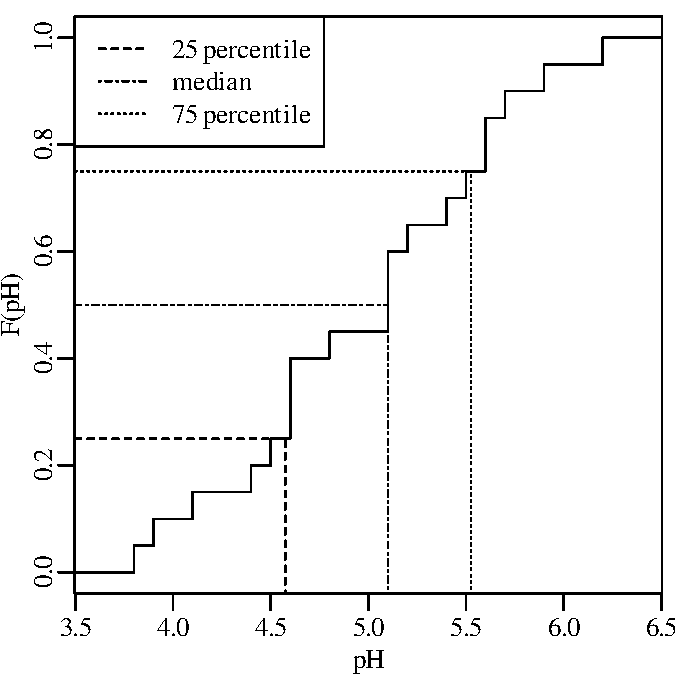
\includegraphics[width=\textwidth]{../figures/IQRpH.pdf}
\end{minipage}
\begin{minipage}[t][][t]{.6\textwidth}
  \captionof{figure}{ECDF of the pH data with indication of the three
    quantiles, namely the 25 percentile, median and 75 percentile.
    The Interquartile Range (IQR) is defined as the difference between
    the 75 and 25 percentiles. This is 1 pH unit in this example.  The
    standard deviation and Median Absolute Deviation are $s[x] = 0.65$
    and MAD = 0.5 pH units, respectively.}
\end{minipage}

\section{Shape}
\label{sec:shape}

The \textbf{skewness} of a distribution is defined as:
\begin{equation}
  \mbox{skew}(x) = \frac{1}{n \cdot s[x]^3}\sum\limits_{i=1}^{n}(x_i-\bar{x})^3
  \label{eq:skew}
\end{equation}

To assess the meaning of this new summary statistic, let us plot the
pH and Ca/Mg datasets alongside the distribution of Covid-19 death
rates (in deaths per 100,000 people) in the UK:\medskip

\noindent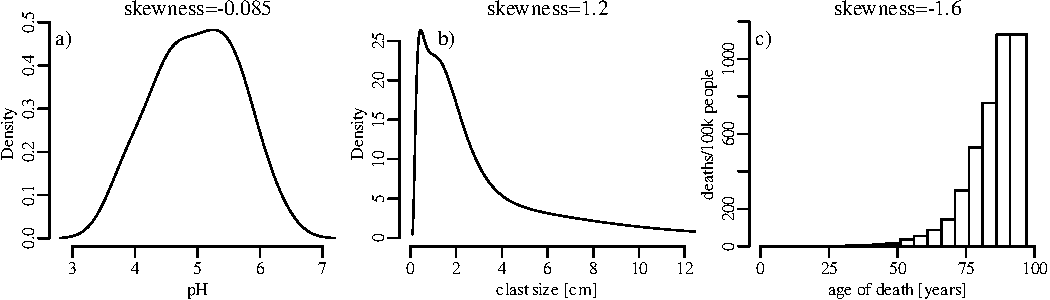
\includegraphics[width=\textwidth]{../figures/skewness.pdf}
\begingroup \captionof{figure}{a) the frequency distributions of pH
  data is symmetric and is characterised by a near zero (but ever so
  slightly negative) skewness; b) the Ca/Mg measurements are
  positively skewed, i.e. they heavily lean towards small values with
  a heavy `tail' of higher values; c) finally, the distribution of
  Covid-19 death rates in the UK for the year 2020 is negatively
  skewed: old people are much more likely to die of covid than young
  people.\medskip} \endgroup

\section{Box-and-whisker plots}
\label{sec:boxplots}

A box-and-wisker plot is a compact way to jointly visualise the most
important summary statistics in a dataset:

\begin{enumerate}
\item a box is drawn from the first to the third quartile (i.e. from
  the 25 to the 75 percentile);
\item the median is marked by a line in the middle of the box;
\item two lines extend from the box towards the minimum and maximum
  value, ignoring outliers (as defined next);
\item any points that fall more than 1.5 times the IQR below the first
  quartile, or more than 1.5 times the IQR above the third quartile
  are marked as outliers.
\end{enumerate}

\noindent\begin{minipage}[t][][b]{.45\textwidth}
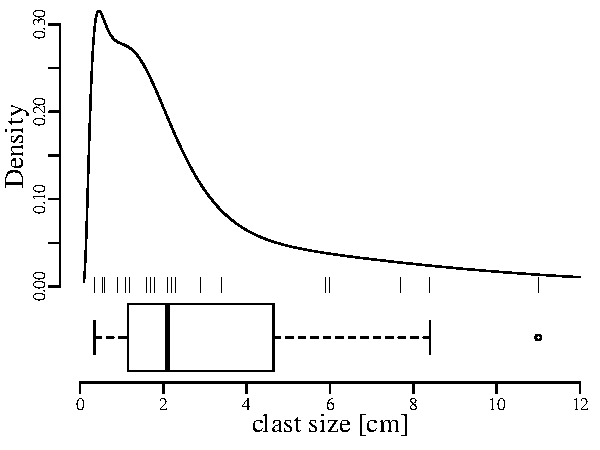
\includegraphics[width=\textwidth]{../figures/boxplot.pdf}
\end{minipage}
\begin{minipage}[t][][t]{.55\textwidth}
  \captionof{figure}{KDE (top) and box-and-whisker plot (bottom) of
    the clast size data. The width of the box marks the IQR.  The
    whiskers extend to the minimum and maximum value, excluding a
    single outlier which, at $\sim$11cm, is more than 1.5 IQR larger
    than the third quartile (75 percentile). The median is offset
    towards the left hand side of the box, indicating the positive
    skewness of the dataset.}
\end{minipage}
